\documentclass{article}
\usepackage{graphicx} % Required for inserting images

\title{HW06}
\author{Riccardo Zucchelli 1984963}
\date{October 2024}

\begin{document}

\maketitle

\section{Introduction}
\textbf{PDM}, or \textit{Password-Derived Moduli} (Figure \ref{fig:pdm}), is a password-based protocol used for mutual authentication and session key generation. This protocol distinguishes itself from other similar protocols by using augmentation systems to make authentication stronger and more resistant to impersonation attacks. 

Many password-based authentication protocols, such as the Extended Key Exchange (EKE), rely on the concept of a shared secret between the client and server. However, one of the major vulnerabilities of this protocol arises in the event of a server data breach. If an attacker gains access to the shared secret, they could exploit this to carry out a variety of attacks. For example, obtaining the password hash (denoted as \( W \)) could allow the attacker to impersonate the user, particularly if the protocol lacks sufficient security measures.

In this scenario, the compromise of the password hash on the server has similar consequences to a direct compromise of the password itself. It could, for instance, lead to the impersonation of the client and facilitate a Man-in-the-Middle (MitM) attack, where the attacker intercepts and potentially alters the communication between the client and server.
\subsection*{The Solution Offered by PDM}
\begin{figure}[h]
    \centering
    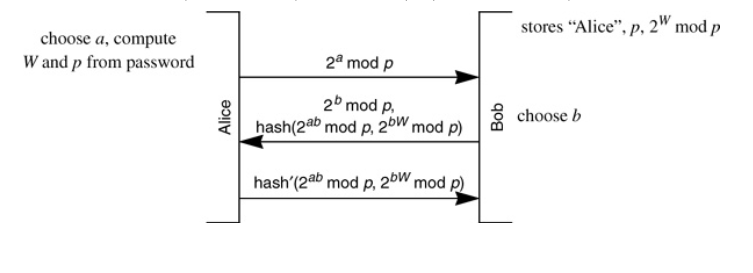
\includegraphics[width=0.8\linewidth]{pdm.png}
    \caption{Password-Derived Moduli protocol}
    \label{fig:pdm}
\end{figure}

The \textbf{PDM} protocol addresses this problem by introducing an \textit{augmentation} mechanism, which makes it more difficult for an attacker to exploit a data breach. This mechanism relies on the use of the\textit{modulo function} along the \textit{discrete logarithm problem} to secure the password-derived value, using it as an authentication method for the password.
As other password protocols do, PDM also enables the secure generation of session keys that can be used to encrypt communication between the client and the server.
\subsubsection*{How does the algorithm work?}
We will focus more on what makes this protocol more secure against impersonation, compared to others.

\begin{itemize}
    \item The server stores the client's identity, along with the prime number \( p \) and the value \( 2^W \bmod p \), and the value will be used in the handshake protocol, specifically in the second handshake message. 
    \item As a session initialization the client uses its password to derive both the prime \(p\) and the value \(W\), then chooses a value \(a\) and sends to the server \(A = 2^a \bmod p\)
    \item The server, which has now calculated its session key, sends back \(2^b \bmod p\). Along that, it sends a "confirmation" of its identity by hashing both the session key and the value \( 2^{pW} \bmod p \).
    \item At this point, the client would confirm that the hash is correct by calculating it and comparing it against the one received by the server, and sends back the hash of the same 2 messages with another algorithm. 

\end{itemize}
To compute \( 2^{pW} \bmod p \), an attacker would need to use \( B^W \bmod p \) or \( (2^W \bmod p)^b \). However, the first method is the only way the client can derive the value, since it has access to \( W \). In this example of server breach, an attacker does not have access to \( W \), which makes it impossible for them to spoof the client's identity just through the knowledge of the stolen data.

\newpage
\section{An example for this algorithm}
We will now calculate 3 different examples of session keys, putting them in a spreadsheet and then evaluating the results by their security level.
Let's hypothesize that p has been generated with a password. As noted by the paper readable here(\texttt{https://typeset.io/pdf/pdm-a-new-strong-password-based-protocol-5cvsd24e04.pdf}) a prime number should be at least of \(p = 700\) bits to be considered safe , which wouldn't be feasable to represent with a table in this homework.

\begin{table}[h]
\centering
\renewcommand{\arraystretch}{1.5}
\begin{tabular}{|l|c|c|c|}
\hline
\textbf{Step}                  & \textbf{Good Example}              & \textbf{Bad Example}              & \textbf{Very Bad Example}        \\ \hline
\textbf{Public Parameters}     & \( p = 104729, g = 2 \)            & \( p = 1009, g = 2 \)             & \( p = 1013, g = 2 \)            \\ \hline
\textbf{Alice's Private Key}   & \( a = 98765 \)                    & \( a = 170 \)                     & \( a = 507 \)                    \\ \hline
\textbf{Bob's Private Key}     & \( b = 45678 \)                    & \( b = 450 \)                     & \( b = 1012 \)                   \\ \hline
\textbf{Alice's Public Key}    & \( A = 2^{98765} \bmod 104729 \)    & \( A = 2^{170} \bmod 1009 = 270 \) & \( A = 2^{507} \bmod 1013 = 1 \)  \\ \hline
\textbf{Bob's Public Key}      & \( B = 2^{45678} \bmod 104729 \)    & \( B = 2^{450} \bmod 1009 = 729 \) & \( B = 2^{1012} \bmod 1013 = 1 \) \\ \hline
\textbf{Shared Secret (Key)}   & \( K = B^a \bmod 104729 \)          & \( K = 729^{170} \bmod 1009 = 16 \) & \( K = 1 \)                      \\ \hline
\end{tabular}
\caption{Diffie-Hellman Key Exchange Examples based on generation of p from the password}
\end{table}

\subsection*{Analysis of the results:}
The first example can be considered good, if we consider for this example infeasible to brute force the private key. Prime is larger than the other ones, along with the chosen private keys. This ensures cryptographic security, and a good randomness value.

The last example, in contrast, is very bad because of a key mathematical issue stemming from how modular exponentiation works in number theory. When Bob computes his public key \( B = 2^b \bmod p\), the result is 1. This happens because 1013 is prime, and by Fermat's Little Theorem, any integer \(g\) co-prime to 1013, which in this case is fixed to 2,  raised to the power of \(p-1\) (which is 1012) will be congruent to 1 modulo 1013. Since Bob's private key is exactly 1012, his public key becomes 1.
This is a critical problem because when Alice uses Bob's public key to compute the shared secret, she gets \(K=1^a \bmod 1013 = 10\), regardless of her private key \(a\). Similarly, when Bob computes the shared secret using Alice's public key, he gets \(K=A^{1012} \bmod 1013\), which also results in 1 due to Fermat's Little Theorem. This makes the session key completely predictable—any attacker observing the exchange would instantly know the shared secret is 1, effectively breaking the encryption.

\section{Attacks of the PDM in a breach}
In case of a possible breach we need to be sure that all private data, like for example \(W\), is safely protected against an attack. Specifically we want to analyze the case in which there is a database breach at the server level, so that the attacker can gain access to Alice's identity, \(p\) and \(2^W \bmod p\). The attacker knows the result of the modular exponentiation involving a secret exponent W and a prime p. However, the attacker doesn't directly know the value of W (the secret key), and that’s critical for impersonating a client. However, there are still potential strategies an attacker might use to impersonate the client, depending on the vulnerability of the system.

\begin{description}
    \item[1. Brute Force Attack on the Exponent W:] In case the Key-Derivation Function (KDF) is weak, the attacker might attempt to brute-force the secret W. For example, if the prime \(p\) is small (even 512bits could be too small), it may be computationally feasable to check all possible values of \(W\) in a relatively small amount of time. Another possibility is that, even if \(p\) is large, the secret exponent \(W\) is derived from a small range of values.
    \item[2. Rainbow Table Attack:] This is somewhat similar to the idea of the brute force attack, expanding on that idea and pre-calculating \(p\) and \(W\) from the most common passwords. This is a good method, in the sense that makes it feasible for an attacker to quickly find a big list of passwords from just the knowledge of all breached values of \(2^W \bmod p\), given enough physical space to store it.
\end{description}
Ultimately, PDM improves the assurance of mutual authentication between two parties. It ensures that both the server and the client can trust each other's identity without exposing sensitive information, like the password itself, to potential attackers. The method is efficient because it minimizes the overhead of traditional key management systems while maintaining high security standards, making it an ideal choice for modern, password-based authentication systems.
\end{document}
